\chapter{OSDOCR Filsofia}
\label{cap_osdocr_filosofia}

Neste capítulo é realizada uma reflexão sobre o problema e as consequentes propostas que são deste retiradas. Serão descritas decisões e modelos fundamentais da solução, assim como a arquitetura desta. 

\section{O problema}

Na sua essência, o problema abordado pode ser descrito como a aquisição de resultados não satisfatórios na aplicação de OCR sob documentos antigos com texto estruturado. 

Como se analisou no capítulo \ref{cap_estado_arte}, estes resultados podem ser melhorados através de múltiplas interações em múltiplas partes do processo do reconhecimento de texto: quer seja antes deste ser realizado, através de processamento de imagem; durante a deteção de texto, através da configuração proposta ao motor OCR; ou após através do tratamento dos resultados e do texto.

Estas diferentes interações são, na generalidade, aplicações sobre um input inicial de forma a transformá-lo, consequentemente resolvendo particularidades deste. Exemplos disto são: aplicação de técnicas de binarização que reduzem ruído ou imperfeições numa imagem; melhoria de resolução de uma imagem; correções ortográficas de texto; etc. Estas interações, podem então ser consideradas como um conjunto de ferramentas que podem ser aplicadas ao input do nosso problema de forma a abordar diferentes defeitos deste de acordo com as suas características; até porque, como também foi descrito para algumas destas, a sua utilização indiscriminada pode deteriorar, ao invés de melhorar, o produto final. As ferramentas comummente utilizadas não são explicitamente dedicadas ao problema de OCR em concreto, aumentando a sua utilidade e adaptabilidade para outras situações.
Tal reforça o intuito base do trabalho, da criação de um toolkit que proporcione um conjunto de funcionalidades independentes, com a intenção final de procurar melhorar os resultados da transcrição de texto.

Podemos então declarar aqui uma primeira proposta: 

\highlight{Proposta 1: A solução para o problema deve ser composta por um conjunto de ferramentas independentes, i.e. um toolkit.}[\normalsize]

Durante a análise do estado da arte, notou-se que para soluções para o problema de melhorar a aplicação de OCR, um processo com 3 partes principais pode ser identificado, sendo estas: pré-processamento de OCR, composto por processamento do input para realização de OCR, usualmente uma imagem; OCR, configurando o motor de OCR de acordo com as características do input, como a linguagem esperada do texto ou o dpi da imagem; pós-processamento de OCR, aplicando transformações nos resultados como, remover blocos de ruído, ordenar blocos identificados ou aplicar correções no texto. 

\begin{figure}[H]
     \centering
     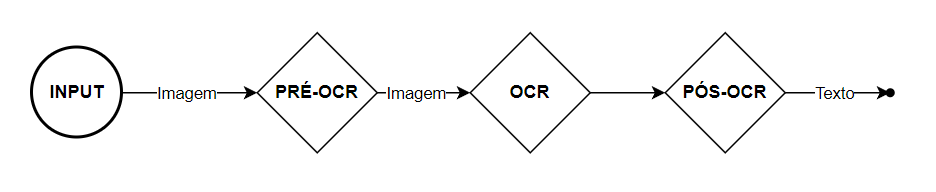
\includegraphics[width=1\textwidth]{images/diagramas/pipeline_alto_nivel.png}
     \caption{Aplicação de OCR com passos para melhoria de resultados}
     \label{fig:pipeline_high_level}
\end{figure}
 
Observando a figura \ref{fig:pipeline_high_level}, podemos identificar que a estrutura das soluções para aplicação de OCR é uma pipeline.

Estas pipelines podem ser elaboradas como uma sequência de aplicações das ferramentas acima mencionadas, como por exemplo:

\begin{figure}[H]
	\centering
	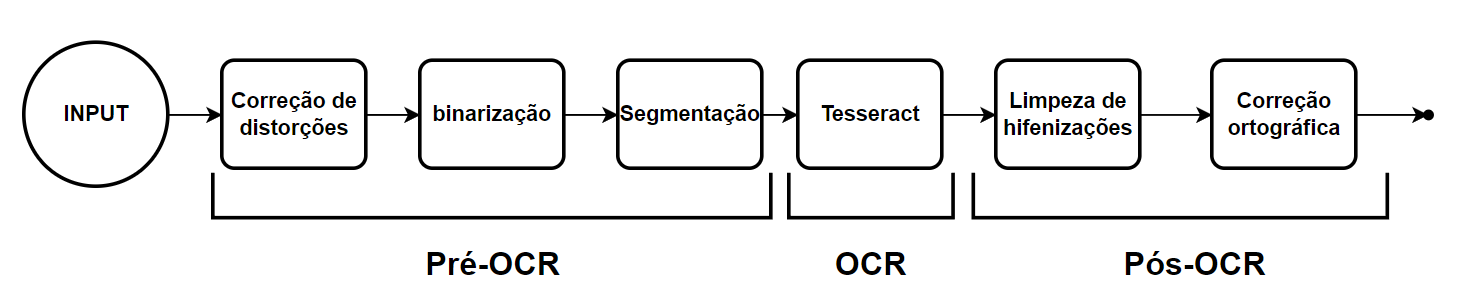
\includegraphics[width=1\textwidth]{images/diagramas/pipeline_exemplo.png}
	\caption{Exemplo de pipeline de aplicação de OCR}
	\label{fig:pipeline_example}
\end{figure}
 
 
Assumindo então a proposta da criação de um toolkit, e a necessidade de verificar a eficácia deste e criar casos de uso deste, torna-se claro que será útil o desenvolvimento de uma pipeline de aplicação de OCR, que faça uso do toolkit desenvolvido, assim como de outras ferramentas disponíveis e que abordem questões em falta no toolkit.

Seguindo o estudo realizado, esta pipeline será composta por 3 partes principais: pré-OCR, OCR e pós-OCR.


% proposta de pipeline

% proposta de pipeline composta por 3 areas principais, processamento de imagem, OCR, processamento de resultados


\highlight{Proposta 2: A solução para o problema deve possuir uma pipeline de aplicação de OCR que faça uso da toolkit desenvolvida.}[\normalsize]

\highlight{Proposta 3: A pipeline desenvolvida deve ser composta por 3 partes principais: pré-processamento de OCR, OCR e pós-processamento de OCR.}[\normalsize]
 
 
Como discutido, o uso de ferramentas independentes é interessante devido ao facto que diferentes inputs irão necessitar de tratamentos distintos de forma a obter os melhores resultados. Desta forma, é interessante que a pipeline desenvolvida não seja totalmente sequencial, de modo a aumentar a sua utilidade.

% proposta de pipeline composta por blocos opcionais

\highlight{Proposta 4: A pipeline deverá ser configurável. Permitirá, dentro dos blocos disponíveis, escolher aqueles que são aplicados.}[\normalsize]

Esta pipeline, seguindo a estrutura explicada de aplicação de OCR, apresentará 3 partes principais onde, a primeira - pré-OCR - irá lidar com um input do tipo imagem e terá como output uma imagem; a segunda - OCR - terá como input uma imagem e devolverá os resultados de OCR; e a última - pós-OCR - irá ter como input os resultados de OCR, e terá como output a transcrição do texto da imagem.

Nota-se uma ambiguidade no output da 2º parte e no input da 3º, os resultados de OCR. Tal, deve-se ao facto de motores OCR, como o Tesseract, permitirem vários tipos de output. É então relevante a criação de um estrutura de dados universal para a representação de resultados OCR.

Como estudado no capítulo \ref{cap_estado_arte}, tais representações já possuem um standard um formato de ficheiro, como \textbf{HOCR}, portanto a estrutura de dados escolhida deve ser baseado nestes, ou ser convertível para o standard.

% proposta de estrutura de dados unica para a represantacao de resultados OCR

\highlight{Proposta 5: Criação de uma estrutura de dados universal para a representação dos resultados de OCR.}[\normalsize]

\highlight{Proposta 6: A estrutura de dados universal para a representação dos resultados de OCR deve ser baseada ou convertível num formato standard.}[\normalsize]


No estudo do estado da arte, foi possível compreender que a criação de algoritmos ubíquos para todos os tipos de documentos é um empreendimento com diminutas chances de sucesso, sendo que para muitos problemas, como por exemplo o cálculo da ordem de leitura, mesmo focando num só tipo de documento como jornais, os resultados podem não ser satisfatórios devido à diversidade de estruturas existentes. Consequentemente, é esperado que a pipeline não seja sempre suficiente na resolução do problema. 
Deste modo, servindo também como outro caso de uso do toolkit, a criação de uma ferramenta que permite ao utilizador um maior manuseamento dos resultados de OCR é uma proposta para a solução. 

Tendo em conta a forte qualidade visual desta área de trabalho, onde se procura processar e analisar imagens de documentos, a utilidade e usabilidade desta ferramenta de edição é elevada ao definirmos que o editor seja gráfico.

% proposta de editor de estrutura de dados para realizacao de afinações manuais

\highlight{Proposta 7: A solução do problema deverá possuir um editor gráfico dos resultados de OCR, que permita aplicar ferramentas propostas pelo toolkit.}[\normalsize]


% apanhado das proposta

Em suma, as propostas definidas para o desenho da solução são:

\begin{enumerate}[label=\textbf{\arabic*}]\setlength\itemsep{-0.8em}
	\item A solução para o problema deve ser composta por um conjunto de ferramentas independentes, i.e. um toolkit.
	\item A solução para o problema deve possuir uma pipeline de aplicação de OCR que faça uso da toolkit desenvolvida.
	\item A pipeline desenvolvida deve ser composta por 3 partes principais: pré-processamento de OCR, OCR e pós-processamento de OCR.
	\item A pipeline deverá ser configurável. Permitirá, dentro dos blocos disponíveis, escolher aqueles que são aplicados.
	\item Criação de uma estrutura de dados universal para a representação dos resultados de OCR.
	\item A estrutura de dados universal para a representação dos resultados de OCR deve ser baseada ou convertível num formato standard.
	\item A solução do problema deverá possuir um editor gráfico dos resultados de OCR, que permita aplicar ferramentas propostas pelo toolkit.
\end{enumerate}


\section{Modelos}

\section{Arquitetura da solução}